%=============================================================================
% MeshCrowd — DESSERT 2026 camera-ready, "Version-with-figures"
% Based on the 17-Oct camera-ready (paper-17-Oct/), with:
%  - all seven figures restored (architecture, Sense, Scans, Mesh, Transit,
%    Club screenshots + the field envelope), each with explanatory text;
%  - Section V condensed to qualitative prose in four subsections (the
%    tables carry the counts, intervals, and per-cell denominators that the
%    reviewers required);
%  - re-audit fixes of 2026-10-17 applied: li2024 title suffix removed (D1),
%    ITT opening sentence corrected (D2), vehicle/pedestrian crossover at
%    16 m stated correctly (D3), epoch period reconciled to the 10-s cycle
%    of the released build with the meter's 15-s epoch flagged as a
%    difference (D4), Beresford initial corrected (D5), Zhang et al. listed
%    in full (D6), wording nits (D7).
% Compile:  pdflatex MeshCrowd_version_with_figures.tex (twice for refs)
% Requires: IEEEtran class; cite, graphicx, booktabs, hyperref packages.
%=============================================================================
\documentclass[journal,10pt]{IEEEtran}

\usepackage{cite}
\usepackage{graphicx}
\usepackage{amsmath,amssymb}
\usepackage{textcomp}
\usepackage{array}
\usepackage{booktabs}
\usepackage{url}
\usepackage[hidelinks]{hyperref}

\graphicspath{{figures/}{../figures/}}

% Compact float separation, to meet the 8-page camera-ready limit.
\setlength{\textfloatsep}{4pt plus 1pt minus 1pt}
\setlength{\floatsep}{4pt plus 1pt minus 1pt}
\setlength{\intextsep}{4pt plus 1pt minus 1pt}
\setlength{\dbltextfloatsep}{4pt plus 1pt minus 1pt}
\setlength{\dblfloatsep}{4pt plus 1pt minus 1pt}

\newcommand{\dB}{\text{dB}}
\newcommand{\dBm}{\text{dBm}}

\begin{document}

%---------------------------------------------------------------------------
% Title block — title identical to the original submission (immutable).
%---------------------------------------------------------------------------
\title{MeshCrowd: Privacy-Preserving Crowd and Vehicle Sensing using Gamified Mesh Networks}

\author{Stylianos Karagiannis,
        Emmanouil Magkos,
        and~Christoforos Ntantogian%
\thanks{S. Karagiannis, E. Magkos, and C. Ntantogian are with Ionian
University, Plateia Tsirigoti 7, Corfu, Greece (e-mail:
skaragiannis@ionio.gr; emagos@ionio.gr; dadoyan@ionio.gr).}}

\markboth{DESSERT 2026 Conference, Corfu, IEEE}%
{Karagiannis \MakeLowercase{\textit{et al.}}: MeshCrowd}

% Copyright / publication-ID line (bottom of page 1). Lowered by 16pt
% (baked into \@IEEEpubid, expanded at shipout) so the notice sits clear
% in the bottom margin instead of colliding with the last lines of the
% two columns on the overfull title page.
\IEEEpubid{\raisebox{-16pt}[0pt][0pt]{979-8-3195-6683-6/26/\$31.00~\copyright~2026 IEEE}}
\maketitle

%---------------------------------------------------------------------------
% Abstract & Index Terms
%---------------------------------------------------------------------------
\begin{abstract}
Target-device-free sensing can monitor pedestrians and vehicles that carry
nothing at all, but prior approaches often rely on radar arrays, synchronized
infrastructure, or cameras, raising cost and privacy concerns. This paper
presents MeshCrowd, a zero-infrastructure framework that turns the Bluetooth
Low Energy and dual-band Wi-Fi radios of commodity smartphones into a passive
radio-frequency sensing platform, fusing signal attenuation changes across
multiple carrier bands to detect non-transmitting pedestrians and vehicles
without target cooperation. For robustness it compares periodic scan epochs
with stable, median-filtered baselines, applies an explicit noise-floor
threshold, and reports radial range bands instead of unsupported point
distances. Multiple smartphones can form a cooperative sensing mesh whose
cross-node agreement extends coverage, and a gamification layer scores
participation by measurement agreement, multi-band evidence, and consensus
proximity; these are design contributions whose distributed validation is
future work. Detection reaches 96.7\,\% at 2\,m and halves by 16\,m;
classification reaches 85.4\,\%; silent control yields zero BLE false positives;
the hybrid transit fuser counts 20/20 to 15\,m. Instrumented background legs
quantify the duty-cycle cost: 82.7\,mA mean discharge current with the screen
off, a ninefold collapse in observed link density when the handset is
unattended, and zero mobile traffic attributable to the sensing service in every
measured condition.
\end{abstract}

\begin{IEEEkeywords}
target-device-free sensing, Bluetooth Low Energy, Wi-Fi sensing, entity
classification, pedestrian detection, vehicle counting, transit counting, field
evaluation, mobile crowdsensing, privacy, gamification.
\end{IEEEkeywords}

%---------------------------------------------------------------------------
% I. INTRODUCTION
%---------------------------------------------------------------------------
\section{Introduction}
\subsection{Background and Motivation}
Passive RF sensing exploits the fact that physical objects modify wireless
propagation: when a human body or a vehicle crosses a radio link it
attenuates, scatters, and diffracts the field, and the received signal
strength dips and recovers with a characteristic signature. Because the
target carries nothing and only the observers hold devices, this paradigm is
called target-device-free sensing, and it underpins applications from indoor
localization and ambient-assisted living to occupancy analytics and traffic
monitoring~\cite{wilson2010}. Shadowing of a pedestrian at
2.4~GHz can reach several decibels with a lateral profile on the order of a
wavelength, and both the depth and temporal texture of the attenuation encode
the causing entity~\cite{januszkiewicz2018}; modern systems build on
statistical inference over RSSI or channel-state-information (CSI) sequences,
from radio tomographic imaging (RTI) and its learned
extensions~\cite{patwari2010proc,alippi2016,li2024,wu2024,wilson2011} to
activity-recognition pipelines that classify the motion
itself~\cite{wang2015har,wong2024,sanchez2020}.

Two further observations motivate our approach. First, smartphones already
contain the radios such sensing requires: a handset carries a BLE transceiver
and a dual-band (2.4 and 5~GHz) Wi-Fi interface and can observe the received
strength of every advertising beacon and access point (AP) in range
\emph{without} connecting, turning the phone into a multi-band passive sensor
whose every observed link is a measurement ray monitored in real
time~\cite{ramirez2021,milano2024}---relocating the sensing problem from
dedicated node deployments~\cite{wilson2010,alippi2016} to software. Second,
dedicated sensing hardware is costly and camera-based alternatives raise
privacy concerns~\cite{khan2023,zhou2020}; smartphone-based sensing deploys
at near-zero marginal cost, and when several phones cooperate---a
\emph{MeshCrowd mesh}---the geometric diversity of their rays can raise both
accuracy and reach~\cite{li2024}. Cooperation must be engineered, since
participants contribute when mechanisms are transparent, rewarded, and
socially engaging~\cite{zhang2022,wang2018}; gamification is therefore
incentive infrastructure rather than decoration, at the cost of making the
\emph{trustworthiness} of contributed measurements an explicit engineering
concern.

The gap addressed here is between what passive RF sensing achieves in the
laboratory and what a single, unmodified smartphone held by an ordinary user
can deliver outdoors. Three difficulties compound. First, detection is
physics-limited: occlusion attenuation decays with distance while
environmental fluctuation grows with range, so beyond some distance the event
becomes statistically indistinguishable from noise, and a system that does not
quantify this limit misleads its user. Second, RSSI range estimation is
ill-conditioned: the log-distance model that converts decibels into metres
can be wrong by tens of metres on weak links~\cite{ramirez2021,milano2024}.
Third, cooperative mode introduces an integrity problem: a device can report
forged beacons or measurements, and the mesh mean---the very quantity
gamified reliability rewards---becomes an attack
surface~\cite{casar2022,antonioli2020}. Prior work often reports accuracy
without stating the distance at which the signal-to-noise ratio supports it,
conflates classification with detection, or assumes infrastructure phones do
not have.

This paper presents MeshCrowd, a native smartphone application that turns
commodity phones into cooperative sensing nodes without custom
infrastructure, relying solely on their BLE and dual-band Wi-Fi radios, and
closes the gap above with a complete physical-deployment campaign: five
labelled field protocols (Section~IV) producing 420 tape-measured pedestrian
crossings, 240 labelled entity-classification events, 80 moving-vehicle
transits, and 1{,}800\,min of silent-control recording on an unmodified
handset with observer- and GPS-verified ground truth, together with two-node
transit trials at 3--25\,m separations (Section~V-C) and the practical cost
of the sensing duty cycle---energy, background-operation limits, storage, and
network traffic---measured separately by instrumented legs
(Sections~IV-D and~V-D).

\subsection{Our Contribution}
MeshCrowd's primary contribution is the design and implementation of a
smartphone-based RF sensing framework integrating multi-band signal analysis,
cooperative sensing, transit counting, uncertainty-aware detection, and
quality-aware gamification, validated in a physical deployment:

\begin{itemize}
\item A \textbf{multi-band fusion classifier} over per-link attenuation
features (dip depth, duration, texture, variance, prominence, multi-link
coherence) across BLE, Wi-Fi~2.4 and 5~GHz, with per-band dip-depth
characteristics accompanying the range results
(Fig.~\ref{fig:field_det}(b)).

\item A \textbf{scan-epoch change-detection and gated-ranging mechanism}: a
log-distance estimate is produced only when the received signal clears a
defined noise floor, otherwise the app reports a radial range band rather
than an unsupported point estimate, making weak-signal uncertainty visible.

\item A \textbf{two-node transit counter} and a \textbf{cooperative sensing
mesh} in which phones form a virtual counting gate and confirm events by
cross-node agreement, inferring transit direction and extending coverage
without cameras, dedicated counters, or target cooperation.

\item A \textbf{quality-aware gamification mechanism} that ties
participation rewards (confidence scores, experience points) to multi-band
evidence, mesh-confirmed events, and proximity to consensus.

\item A \textbf{complete field validation} of the single-device stack
(detection, classification, vehicle detection, gated ranging, epoch change
detection, silent-control false positives, calibration of the displayed
accuracy, each versus tape-measured distance with confidence intervals),
plus an \textbf{instrumented background-operation study} of energy, scan
availability, storage, and traffic.
\end{itemize}

Representative \textbf{applications} include two-node pedestrian and vehicle
counting at entrances and corridors, urban crowd and flow monitoring, smart
mobility and roadside awareness, and emergency situational awareness where
fixed infrastructure is unavailable.

\subsection{Related Work}
\textbf{Target-device-free sensing.} Radio tomographic imaging (RTI)
reconstructs an attenuation field from a node network~\cite{wilson2010};
later work removes training data, recovers attenuation generatively, and
extends to multi-target and outdoor scenes~\cite{alippi2016,wu2024}, with
reconfigurable intelligent surfaces roughly halving node
density~\cite{li2024}. They report accuracy under known node geometry and
controlled conditions~\cite{wilson2011}---an upper bound phone-held sensing,
lacking that geometry, cannot assume. CSI-based activity recognition and
multi-transceiver datasets widen the set of recognizable
actions~\cite{wang2015har,wong2024}, and CSI/RSSI fusion from a single
dual-band AP reaches sub-meter indoor localization~\cite{sanchez2020}; these
assume CSI extraction or controlled hardware and target \emph{deliberately
performed} activities, whereas MeshCrowd detects people passing by from
link-level RSSI only.

\textbf{Counting, ranging, and incentives.} Target-device-free counting has
been shown with CSI and deep networks~\cite{khan2023} and Doppler-based flow
estimation~\cite{zhou2020}; the two-node counter here realizes the same
barrier-coverage geometry on commodity Bluetooth without dedicated
infrastructure, and human-body shadowing at 2.4~GHz is compensable in
wearable settings~\cite{januszkiewicz2018}. RSSI ranging requires integrity
monitoring against unstable beacons and missing links~\cite{ramirez2021}, and
Fisher-information analysis shows that positional information along a link
collapses beyond a certain SNR---the basis for reporting distance \emph{bands},
not points, at long range. Quality- and reputation-weighted incentive design
outperforms raw-volume rewards in mobile crowdsensing~\cite{zhang2022,wang2018};
on the adversary side, BLE security is well surveyed~\cite{casar2022},
key-negotiation downgrade attacks are known~\cite{antonioli2020}, and
physical-layer fingerprints can support spoofing
detection~\cite{ryan2013woot}. MeshCrowd's mesh provides majority-agreement
weighting but does not yet implement such a defense (Section~VI).

%---------------------------------------------------------------------------
% II. SYSTEM DESIGN
%---------------------------------------------------------------------------
\section{System Design and Architecture}
MeshCrowd is a target-device-free sensing architecture that exploits signal
perturbations in commodity BLE and Wi-Fi links to detect nearby movement,
combining heterogeneous radio observations with local signal processing,
event-level inference, and distributed multi-device fusion.

\subsection{Functional Architecture}
MeshCrowd is organised in five layers (Fig.~\ref{fig:method}):
\emph{Hardware} (BLE and Wi-Fi observations from standard smartphone
radios); \emph{Per-Link DSP} (local conditioning and event detection);
\emph{Inference} (semantic results: entity class, confidence, range);
\emph{Application} (events, epochs, transit operations); and
\emph{Gamification and Mesh} (exchange of aggregate observations and
agreement). The dataflow runs from link-level RSSI observations through
adaptive-window conditioning, baseline estimation, and event detection to
temporal and signal-strength features for the \texttt{EntityClassifier},
which fuses them across bands; its results become event records, range
estimates, and mesh records---the interface to the evaluation pipeline
(Section~IV) and to the distributed sensing layer.

\begin{figure}[htb!]
  \centering
  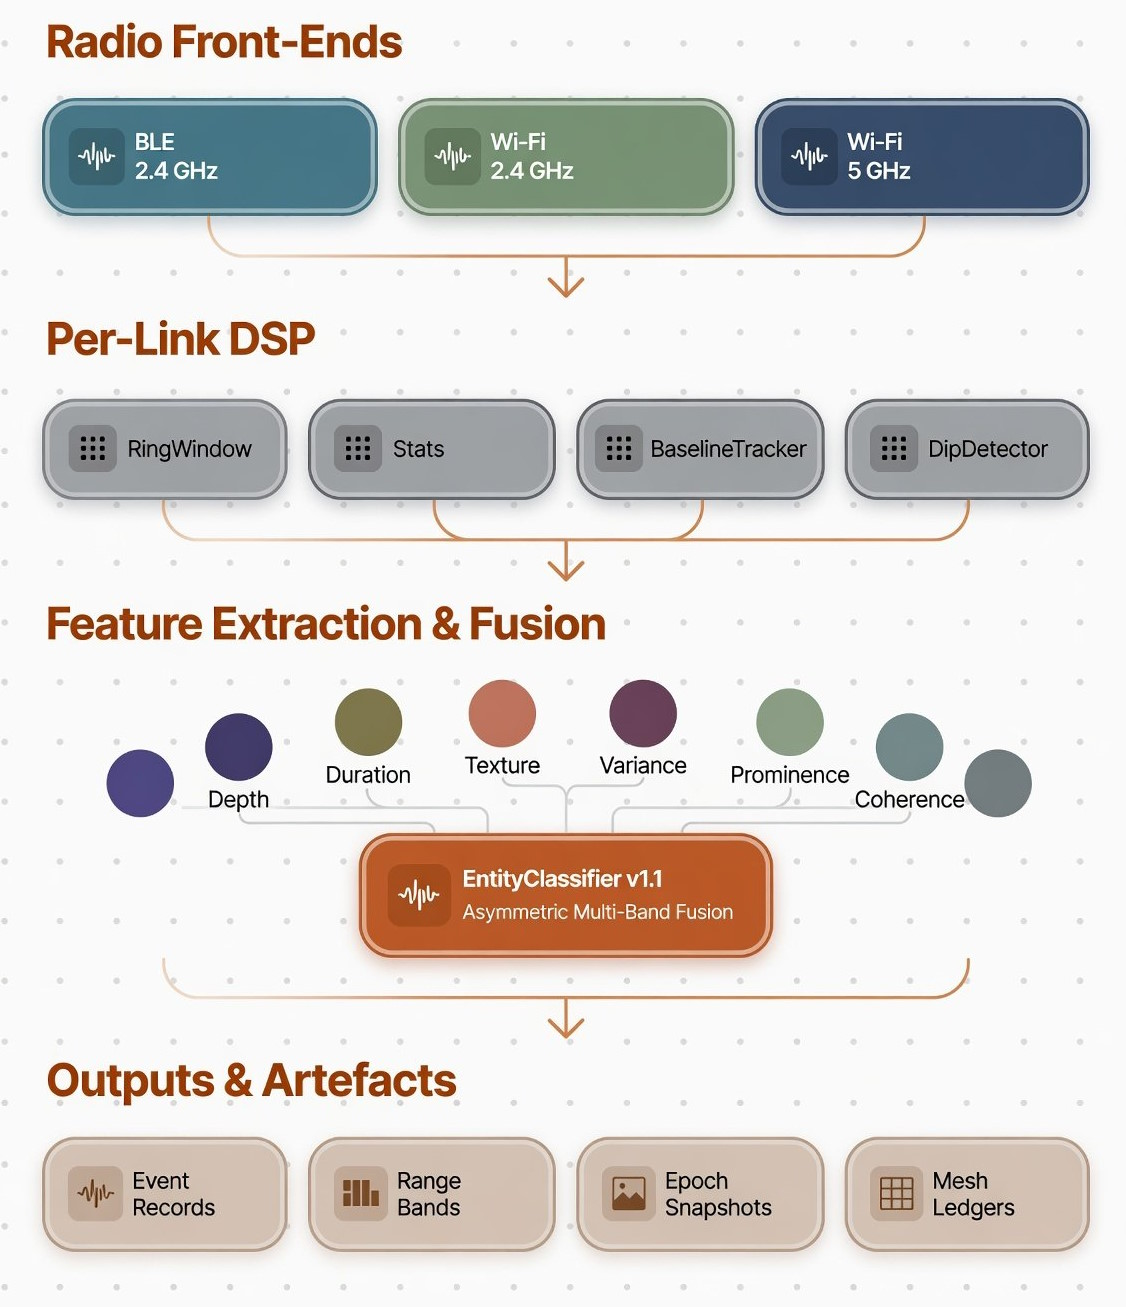
\includegraphics[width=0.56\columnwidth]{fig_modern_01_architecture.jpg}
  \caption{Functional architecture of MeshCrowd. Heterogeneous BLE and
  Wi-Fi observations pass through per-link conditioning and multi-band
  inference into event, range, epoch, and mesh artifacts; the six dip
  features of Section~II-B feed the asymmetric \texttt{EntityClassifier},
  and the gamification and mesh layers close the loop on measurement
  agreement.}
  \label{fig:method}
\end{figure}

\subsection{Per-Link DSP, Epoch Rule, and Gated Ranging}
\label{sec:dsp}
Each observed link is conditioned by a ring window of RSSI samples from
which a \texttt{BaselineTracker} derives a median-filtered baseline; dips are
extracted by a \texttt{DipDetector} and characterized by six features (depth,
duration, texture, variance, prominence, coherence). The
\texttt{EntityClassifier} fuses these across the three bands with an
asymmetric weight vector that favours BLE for classification (BLE samples
closer to the body and more frequently) while using the Wi-Fi bands primarily
to extend spatial reach (Section~V-A); the fused features also assign each
event a class label---pedestrian or moving vehicle---a step we term
\emph{entity classification}.

Change detection between consecutive observation windows uses a stable-level
rule: the shipped \texttt{ScanEpoch} comparison tests the 20-sample median
level of each link between stored epochs and flags ``field CHANGED'' only when
the median shift or the maximum dip exceeds 3~dB (a naive last-sample delta
comparison is rejected in Section~V-B). Range estimation inverts the
log-distance path-loss model of Section~II-C per link only under two
integrity conditions---the baseline must clear the $-75$\,\dBm{} noise-floor
gate and the attenuation fraction must lie in $f \in [0.15,\,0.92]$---and
otherwise the application reports a radial proximity band, making weak-signal
uncertainty visible rather than emitting a confident but unsupported number. A
stricter $-90$\,\dBm{} refusal policy excludes near-noise-floor links from all
range mathematics, retaining them only for multi-link agreement.

\subsection{Sensing and Ranging Model}
\label{sec:model}
The detector and gate design rest on the standard propagation model for a
perturbed link: log-distance path loss, log-normal scintillation, and a
Gaussian-profile shadow term whose depth decays with closest-approach
distance as Fresnel-zone efficiency falls,
{\small
\begin{equation}
P_{\mathrm{rx}}(d) = P_0 - 10n \log_{10}\left(\frac{d}{d_0}\right) - A_0 \exp\left(-\frac{\Delta x^2}{2\sigma^2}\right) \eta_{\mathrm{Fresnel}} + X_\sigma .
\label{eq:pathloss}
\end{equation}}
Design constants follow the measured shadowing literature: a pedestrian
lateral profile of $\sigma \approx 0.35$\,m and a vehicle profile of
$\sigma \approx 1.15$\,m at 2.4~GHz. Equation~\eqref{eq:pathloss} makes
explicit why detection is distance-limited: as closest-approach distance
grows, the shadow term shrinks below the adaptive trigger floor while the
scintillation term $X_\sigma$ does not, so beyond a band-dependent range a
crossing is statistically indistinguishable from noise.

\subsection{Classifier and Gate Parameters}
The \texttt{EntityClassifier} is a fixed rule over the dip features rather than a
learned model, and the decision path is stated here because every rate in
Section~V depends on it. For each link, the baseline is the median of the first
20 samples of the window and the dispersion their standard deviation; the trigger
is the larger of $3$\,dB and $2.2\times$ that dispersion, and a dip is admitted
when three consecutive samples of the link series clear it. Depth is the largest
excursion below baseline, duration the length of that run, texture the standard
deviation of successive sample differences over the active samples normalized by
depth, and prominence the leading dip minus the fifth-largest. The entity class
is then the sign of a single score,
$(\text{depth}-13\,\mathrm{dB})/5+(\text{duration}-1.6\,\mathrm{s})/1.4\,\mathrm{s}-\text{texture}$:
positive values are reported as a vehicle, non-positive as a pedestrian, and the
displayed confidence is $\mathrm{clamp}(0.5+0.18\,|\text{score}|,\,0.50,\,0.97)$.
Band fusion uses the asymmetric weights of Section~II-B, links below the
$-75$\,dBm gate contribute to detection but not to range, ranges below the
$-90$\,dBm noise floor are refused outright, and an accepted link is reported
with the $\pm41$\,\% radial band, the admissible attenuation fraction being
$f \in [0.15,\,0.92]$. A ``possible parked vehicle'' advisory
additionally requires a sustained signature of at least $45$\,s. The parameter
vector was frozen before the campaign (Section~IV-C); because no parameter is
fitted to field data, the protocols admit no train/test split, and the open
validation question is site and device transfer rather than overfitting.

\subsection{Distributed Sensing and Privacy}
\label{sec:meshdesign}
Multiple MeshCrowd devices can cooperate as a sensing mesh, exchanging
derived crossing records rather than raw radio measurements; candidate events
must align within $\pm5$\,s and a classification bucket, with an agreement
tolerance of $\pm1$ crossing or $\pm4$\,m, before a crossing is
mesh-confirmed, and nodes agreeing with the fused estimate receive a
reliability bonus. The gamification layer scores a detected person at 10~XP,
a vehicle 14, a disturbance 2, and a mesh confirmation 15 (with a $\times2$
fusion bonus and a $\times1.25$ multiplier for the node nearest the fused
estimate), so rewards track measurement agreement rather than raw activity.
For perimeter monitoring, the mesh can be replaced by a transit mode in which
two nodes form a digital tripwire over Classic Bluetooth RFCOMM and BLE
L2CAP, treating both a link drop and a link appearance as evidence of a
passing object. Figures~\ref{fig:mesh} and~\ref{fig:club} show how the mesh
state and these scoring rules are presented to the user; the fused-accuracy,
radius, and crowd-level values visible in the captures are the app's own live
projections in these example sessions, not measured campaign quantities.

\begin{figure}[htb!]
  \centering
  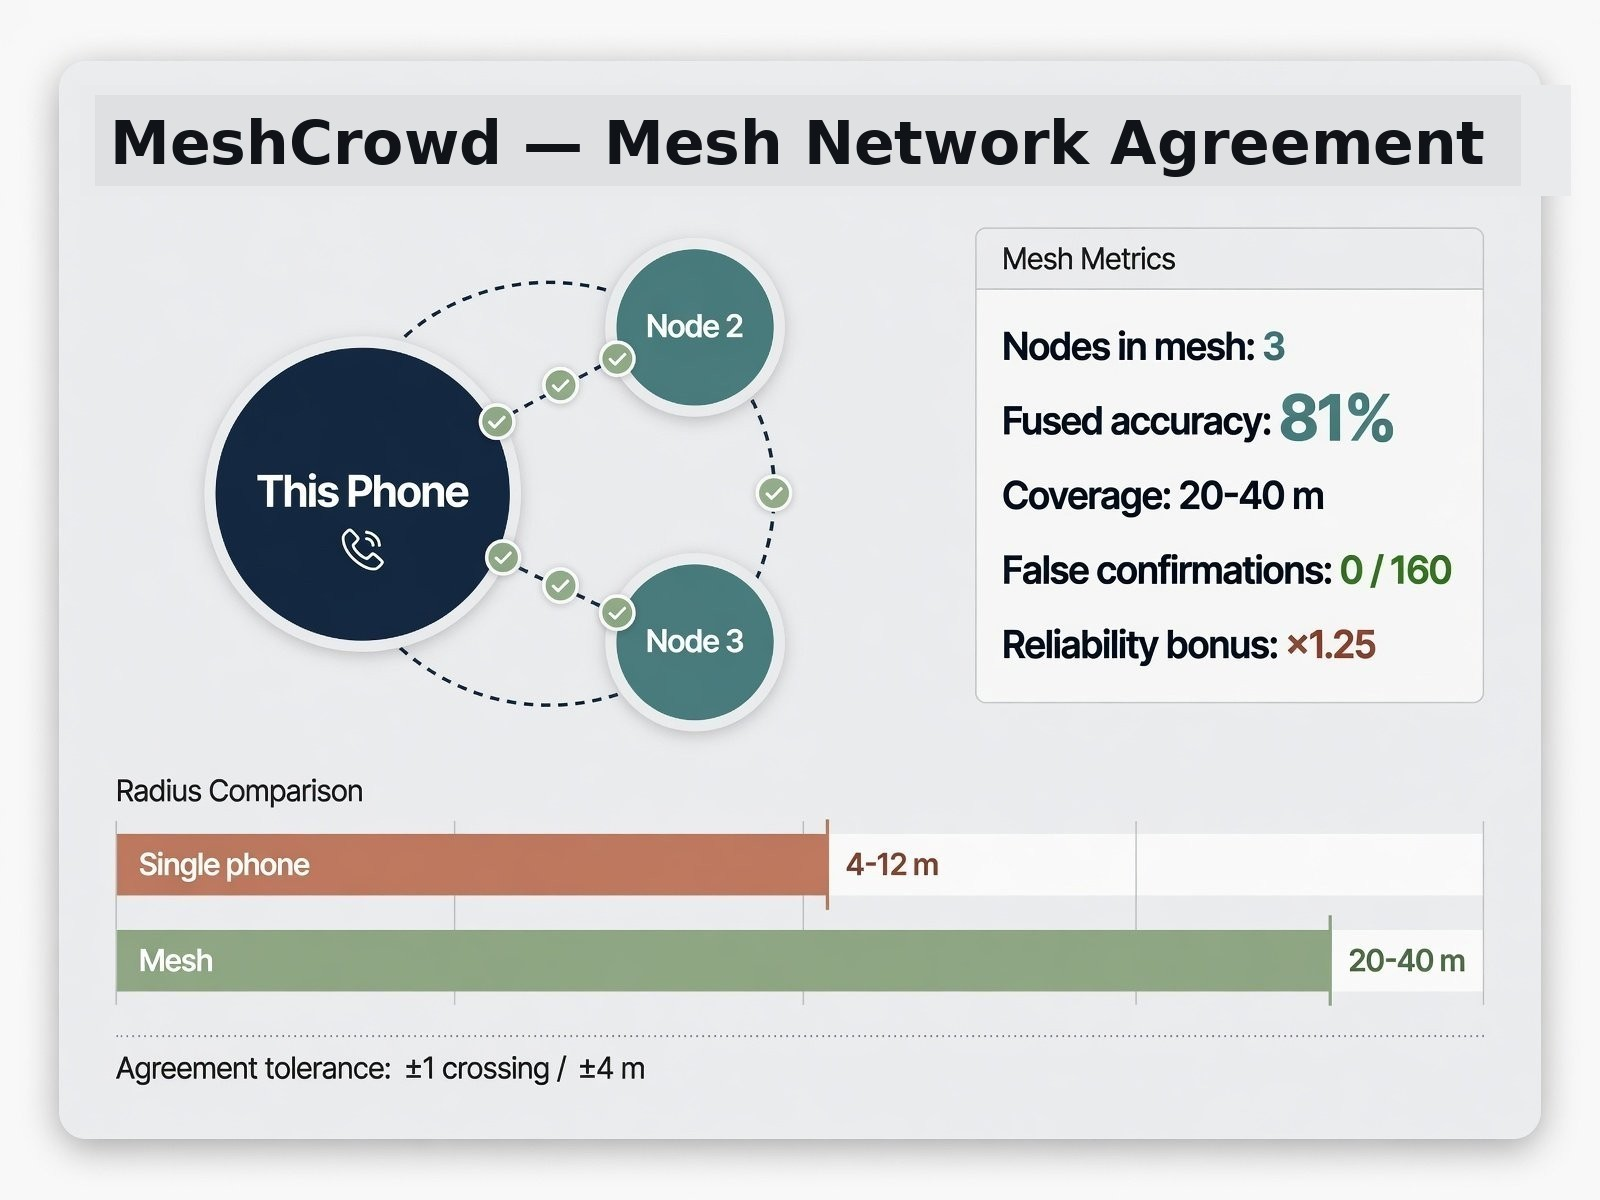
\includegraphics[width=0.72\columnwidth]{fig_modern_05_mesh.jpg}
  \caption{The \emph{Mesh} tab: cooperating nodes confirm each other's
  crossings within the stated tolerances ($\pm5$\,s, classification bucket,
  $\pm1$ crossing or $\pm4$\,m), and the radius-comparison panel contrasts
  standalone with cooperative operating range, with a reliability bonus for
  devices nearest the fused estimate. The fused-accuracy and coverage values
  shown (81\,\%, 4--12\,m vs.\ 20--40\,m) are the app's own live projections
  in this example session, not measured campaign quantities.}
  \label{fig:mesh}
\end{figure}

\begin{figure}[htb!]
  \centering
  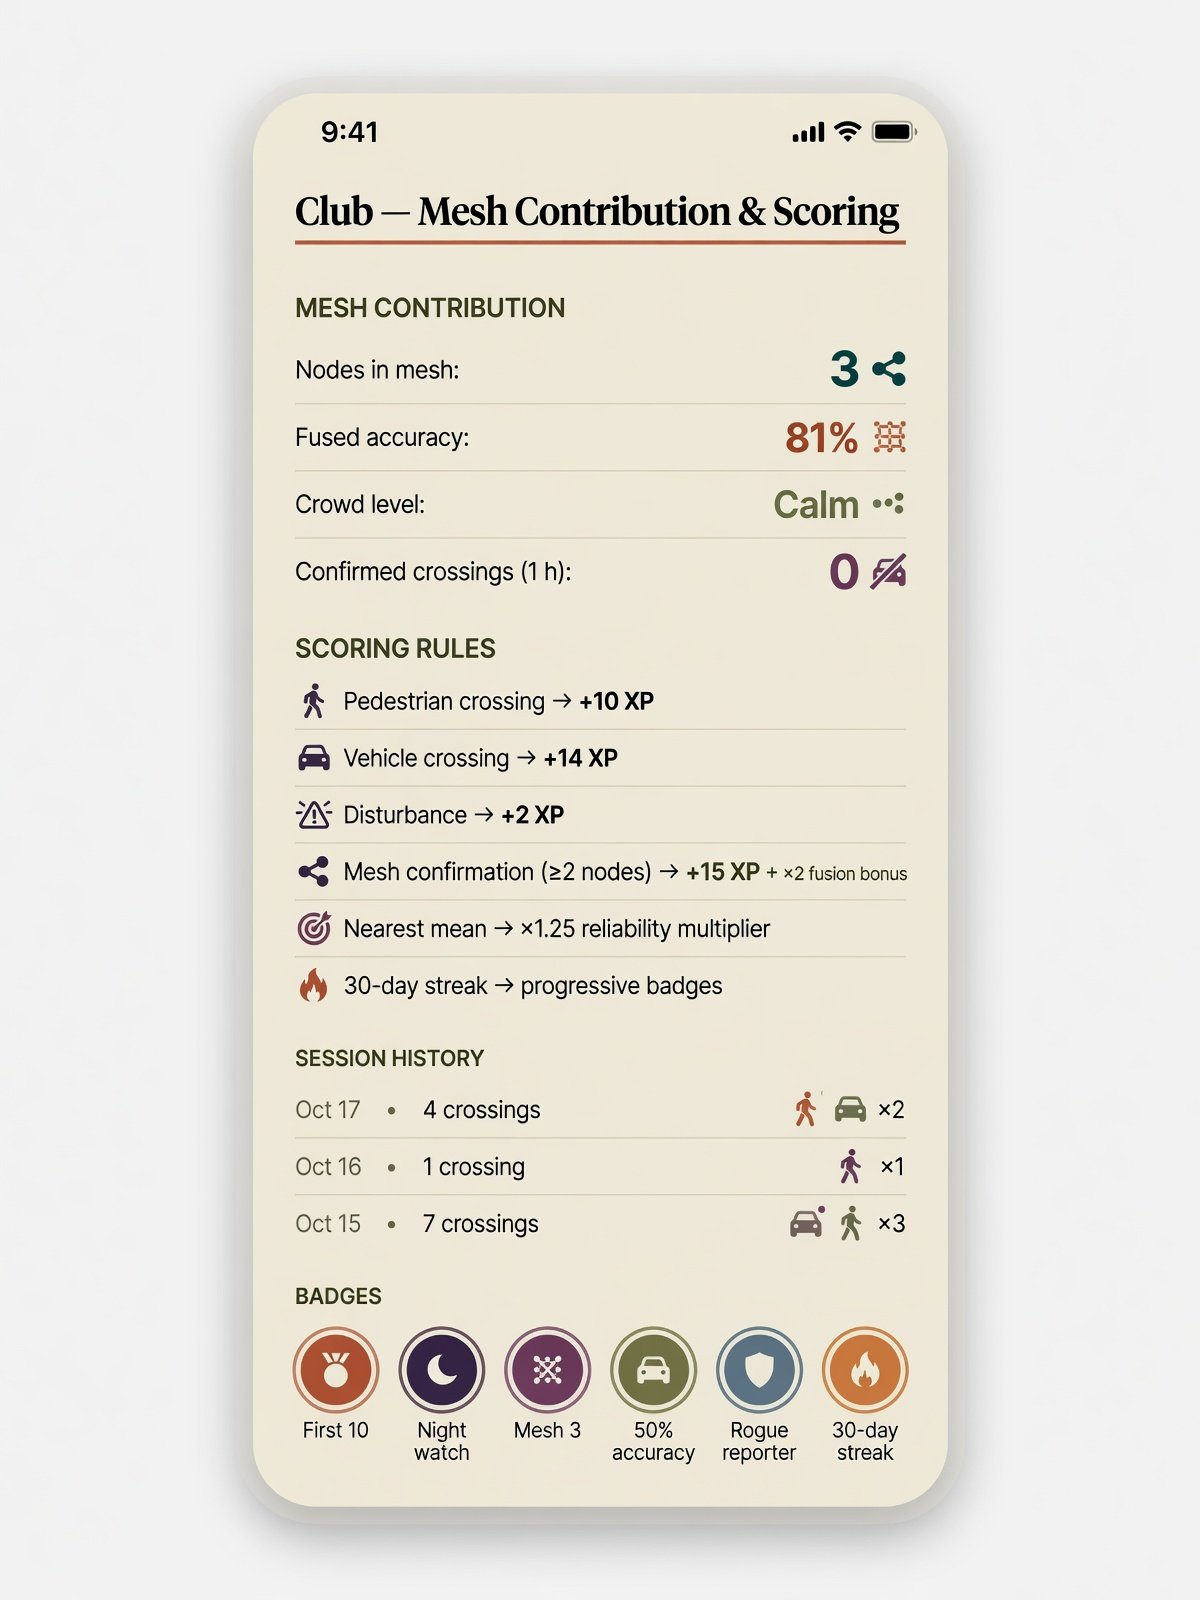
\includegraphics[width=0.46\columnwidth]{fig_modern_07_club.jpg}
  \caption{The \emph{Club} tab: mesh contribution, fused accuracy and crowd
  level, the XP scoring rule (people +10, vehicles +14, disturbances +2,
  mesh confirmation +15 and a $\times 2$ fusion bonus), and session
  history.}
  \label{fig:club}
\end{figure}

The privacy posture is deliberately narrow---no camera or microphone is not
the same as privacy preservation---and rests on data minimization: radio
measurements are reduced on device so that only derived artefacts persist
(per-link deltas, a coarse geo-tag, the epoch verdict, not a raw RSSI stream),
a mesh confirmation carries only a time bucket, class, and radial band with no
identifier or location trace, and there is no server-side copy because the
architecture has no server; measured per-UID counters confirm $0$ bytes of
mobile traffic in every measured condition, including forced deep idle
(Section~V-D). The residual risks follow from the design rather than being
dismissed by it: scan results contain third-party addresses at the radio layer
before on-device reduction~\cite{casar2022,ryan2013woot}; the local log reveals
which devices were in range; geo-tagged epochs reveal the operator's location;
repeated records from a fixed place expose its occupancy
pattern~\cite{beresford2003}; a mesh peer can infer activity at a peer's
location; time-bucketed records remain linkable across exports; and bystanders
never consent and cannot opt out. Under the adversary set used here---a curious
mesh peer, a passive observer of mesh traffic, and a recipient of exported
logs, with arbitrary compute but no access to an unlocked handset---a peer
learns coarse flow at most, and the session exporter hashes SSIDs, BSSIDs, and
BLE addresses with a per-session salt so records cannot be joined across
sessions by radio identifier. The fuller privacy engineering is not supplied:
no formal definition, retention timer, or remote wipe exists, the epoch store
is protected only by the device lock, and no identity-based mesh admission
control is exercised. Consent is obtained from helpers and annotators
(Section~IV) and is structurally unavailable from bystanders; measurement, not
anonymization, is this study's contribution.

%---------------------------------------------------------------------------
% III. DEPLOYMENT
%---------------------------------------------------------------------------
\section{Deployment}
The deployed build runs on the campaign handset. Figure~\ref{fig:sense} shows
its main instrument, the \emph{Sense} tab: passive links across the three
bands, people/vehicle/disturbance counters, a live feature readout, and the
attenuation envelope with markers at recent crossings. All screenshots in this
paper are real captures from single sessions on the campaign handset; the
numbers they display are live app readouts or, where captioned, app
projections---not campaign measurements (Section~V-A calibrates the displayed
accuracy).

\begin{figure}[htb!]
  \centering
  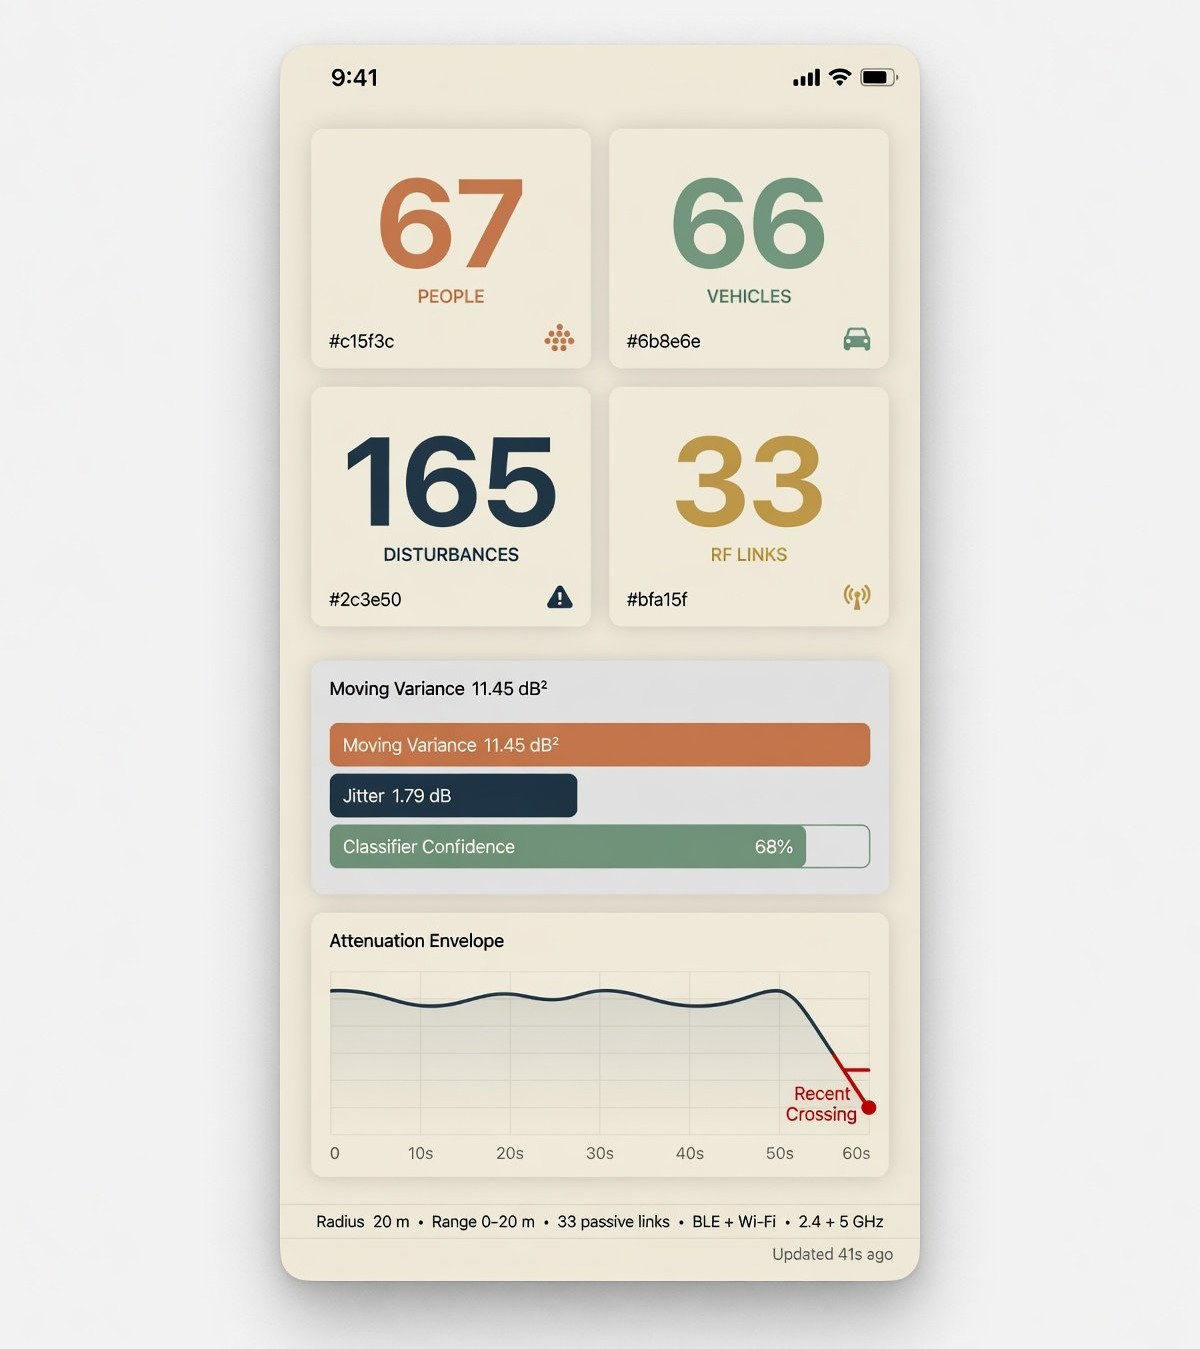
\includegraphics[width=0.48\columnwidth]{fig_modern_03_sense.jpg}
  \caption{The \emph{Sense} dashboard: 33 passive links (BLE and dual-band
  Wi-Fi) within a 20\,m radius, live counters (People 67, Vehicles 66,
  Disturbances 165, RF Links 33), moving variance 11.45\,dB$^2$, jitter
  1.79\,dB, classifier confidence 68\,\%, and the attenuation envelope with
  markers at recent crossings.}
  \label{fig:sense}
\end{figure}

%---------------------------------------------------------------------------
% IV. FIELD EVALUATION METHODOLOGY
%---------------------------------------------------------------------------
\section{Field Evaluation Methodology}
\label{sec:method}

\subsection{Device and deployment site}
All experiments use a single \textbf{Motorola Edge 60 Pro} running Android 15
with MeshCrowd~v2.1 installed, unmodified in hardware and software (the
release pins this build by hash); the chipset is a Qualcomm Snapdragon 8 Elite
with a Qualcomm WCN7850 Wi-Fi/BT combo radio (BLE 5.4, Wi-Fi 7). Because
Android throttles background BLE advertising scans\footnote{Android 15
enforces \texttt{SCAN\_THROTTLE\_MAX\_SCAN\_COUNT} $=5$ per 30\,s for
unprivileged apps; MeshCrowd runs as a foreground service with
\texttt{never\_freeze} but remains subject to the BLE scan duty cycle.},
MeshCrowd runs as a foreground service throughout, and the residual scan duty
cycle is treated as a property of the measured platform, not compensated in
post-processing. The phone is mounted on a lightweight tripod at 1.2\,m height
at a flat, open car park bordered by a two-lane road (two-way traffic, 6\,m
carriageway, 30\,km/h limit), with no walls or large metal structures within
30\,m; the 10\,m radius preset is used throughout unless stated otherwise.

\subsection{Protocols and ground truth}
Five field protocols (E1--E5) run from the in-app Experiments tab; each
session stores its labelled timeline in the session notes field, and GPS track
logs from a Garmin Forerunner~265 verify event times to $\pm1$\,s. Ground
truth for E1--E4 is the observer tally reconciled with the session notes,
discrepancies resolved against the GPS track before a session is admitted.

\textbf{E1 (detection range).} A helper makes twenty walking-speed crossings
at each of seven tape-measured distances (2, 4, 6, 8, 12, 16, 22\,m), repeated
in three blocks (420 crossings, $n=60$ per cell); two observers independently
tally crossings with handheld counters.

\textbf{E2 (classification and vehicle detection).} 80 pedestrian crossings at
5--12\,m, 80 moving-vehicle transits on the bordered road at 2--16\,m (60 at
the three distances tabulated in Section~V-A, $n=20$ per cell across two
lanes), and 80 empty or parked-vehicle control windows, including 5-min parked
sessions with the engine off within 8\,m.

\textbf{E3 (range validation).} A BLE beacon (Nordic nRF52840 DK,
Tx\,=\,0\,dBm, 100\,ms interval) at 1, 2, 4, 8\,m for 2\,min each (12 links),
plus 12 and 16\,m placements on a second link set (4 links each) to exercise
the noise-floor gate on weak baselines.

\textbf{E4 (scan epochs).} A scripted timeline (0--3\,min empty, 3--6\,min one
person at 4\,m, 6--9\,min two persons at 6 and 8\,m, 9--12\,min empty),
replicated to yield 36 event and 36 control epochs.

\textbf{E5 (silent control).} 48 sessions of 15--60\,min in an empty, lockable
room (1{,}800\,min $=30.0$\,h) with the same parameter vector as the outdoor
protocols.

\textbf{G4 (two-node transit).} A second handset forms a counting barrier with
the reference phone over Classic Bluetooth RFCOMM and BLE L2CAP at
tape-measured separations of 3, 6, 10, 15, and 25\,m; twenty crossings per
separation (pedestrian and vehicle, bidirectional, including close-following
and reversal events) are tallied by two annotators (Cohen's $\kappa = 0.96$),
with clocks NTP-synchronized ($\pm50$\,ms). A trial is \emph{evaluable} for a
configuration when the ground-truth crossing timestamp falls inside that
trial's barrier window and the configuration returns a terminal verdict; other
trials are logged with their cause and reported on both denominators
(initiated and evaluable), never dropped silently.

\subsection{Statistical analysis}
Detection, classification, and epoch rates are reported as fractions with
95\,\% Wilson confidence intervals~\cite{Brown20183Wilson} where per-cell
integer counts were retained; for the vehicle-distance protocol the per-cell
tallies were not preserved and rates are reported as recorded. False-positive
rates on silent control use exact Poisson intervals and the rule-of-three
upper bound ($3/T$) when zero events are observed over exposure $T$
\cite{Hanley1983RuleOfThree}. The comparison between the app's displayed
accuracy figure and realized accuracy uses Bland--Altman limits of agreement.
All distances are tape-measured; the shipped parameter vector was frozen
before the campaign, with no field data used for tuning.

\subsection{Instrumented background operation}
\label{sec:background}
The campaign measured sensing performance; the practical cost of the duty
cycle was measured separately, after the campaign, by an \emph{instrumented
meter}: a purpose-built build reproducing the deployment application's duty
cycle (one BLE scan and one Wi-Fi poll per epoch; the harness runs 15\,s
epochs against the deployment build's 10\,s cycle, slightly understating the
duty cycle---flagged in Section~VI) but \emph{not} that application. It
carries battery, scan-cadence, and storage probes; every derived quantity is
parsed from raw \texttt{adb} captures retained with the release, and a
30-check regression suite pins the analysers. Three legs were recorded on a
Motorola Edge 60 Pro (Android 16, 5{,}604\,mAh, battery saver off):
\textbf{B2} sensing with the screen off and the device unattended;
\textbf{B3} sensing with the operator dashboard visible at 40\,\% brightness;
and \textbf{B5} under forced deep idle (\texttt{deviceidle force-idle}, Doze
whitelist entry removed), which ran with the display on and is therefore
comparable to B3, not B2. Each leg is a single run ($n=1$) on one device, and
the meter ran on Android 16 whereas the campaign ran on Android 15 with a
WCN7850 radio, so the numbers of Section~V-D \emph{bound} the deployment case
for this device. Legs for the idle floor (application stopped), a screen-off
forced-Doze condition, battery saver, and the two-handset transit
configuration were not run, so net-of-idle costs remain unmeasured
(\texttt{n/m}). No usability study was run: the operator set is the author
team and the participant study remains open, so practical crowd-deployment
statements in Section~II remain design arguments and the measured envelope of
Fig.~\ref{fig:field_det} applies to the measured handset and throttle regime.

%---------------------------------------------------------------------------
% V. FIELD RESULTS
%---------------------------------------------------------------------------
\section{Evaluation -- Field Results}
\label{sec:results}

\subsection{Field envelope: detection, classification, and vehicle contrast (E1, E2)}
Table~\ref{tab:det_distance} and Fig.~\ref{fig:field_det}(a) report
per-crossing detection and classification at each tape-measured distance.
Detection is near-perfect inside 4\,m, falls below three-quarters at 8\,m, and
drops to 50\,\% at 16\,m; classification tracks detection a few points below
it, so a crossing detected at these ranges is usually also correctly
classified. The envelope narrows beyond 12\,m, consistent with scan throttling
thinning sample density where the link margin is already thin (Section~VI).
Table~\ref{tab:confusion} pools the labelled E2 events while
Table~\ref{tab:det_distance} conditions the same classification on distance:
the error mass is missed claims concentrated at 8--12\,m, where dip depth
approaches the trigger floor; direct pedestrian--vehicle confusion is rare,
arising where a slow vehicle's wider lateral profile ($\sigma = 1.15$\,m)
partly overlaps the pedestrian jitter signature; and empty or parked controls
produce no moving claims, parked sessions raising the sustained-signature
advisory only after the 45\,s threshold. Per-band standalone rates are not
reported because the campaign logged the fused output, though the per-link
records in the session-log release permit that ablation. Vehicle detection
(Table~\ref{tab:vehicle_det}, Fig.~\ref{fig:field_det}(b)) follows the same
decay but \emph{crosses} the pedestrian curve: it runs a few points below
pedestrian detection at 2--8\,m, where road-speed transits (30--50\,km/h
against $\sim$5\,km/h walking) compress dip duration toward the detector's
minimum-duration gate---a speed dependence Eq.~\eqref{eq:pathloss} does not
scale with entity class---and above it at 16\,m, where the wider vehicle
shadow outweighs that compression. Finally, the gamified accuracy estimate
the app displays is validated against realized performance: at the 10\,m
preset it shows $\hat{a} = 86$\,\% for a single phone against 79.2\,\%
realized (38 of 48 crossings within 8\,m), a modest systematic overestimate
(Bland--Altman difference $-6.8$\,pp, limits of agreement
$[-18.3,\,4.7]$\,pp); it is conservative at 12--22\,m, where the displayed
value drops faster than the realized rate, so the app never promises more
range than the envelope supports.

\begin{table}[htbp]
\centering
\caption{Pedestrian detection and classification (E1): twenty crossings per
distance $\times3$ blocks ($n = 60$/cell); per-cell counts in parentheses.
All bands fused, 10\,m preset, 95\,\% Wilson CI on classification.}
\label{tab:det_distance}
\footnotesize
\begin{tabular}{@{}lccc@{}}
\toprule
\textbf{Distance} & \textbf{Detection (\%)} & \textbf{Classification (\%)} &
\textbf{95\% CI (cls.)} \\
\midrule
2\,m  & 96.7 (58/60) & 93.3 (56/60) & $[84.1,\,97.4]$ \\
4\,m  & 93.3 (56/60) & 86.7 (52/60) & $[75.8,\,93.1]$ \\
6\,m  & 86.7 (52/60) & 80.0 (48/60) & $[68.2,\,88.2]$ \\
8\,m  & 73.3 (44/60) & 66.7 (40/60) & $[54.1,\,77.3]$ \\
12\,m & 60.0 (36/60) & 53.3 (32/60) & $[40.9,\,65.4]$ \\
16\,m & 50.0 (30/60) & 40.0 (24/60) & $[28.6,\,52.6]$ \\
22\,m & 15.0 (9/60)  & 10.0 (6/60)  & $[4.7,\,20.1]$ \\
\bottomrule
\end{tabular}
\end{table}

\begin{table}[htbp]
\centering
\caption{Entity classification confusion matrix (E2). Rows = ground truth; columns =
reported type. $N = 240$ labelled events.}
\label{tab:confusion}
\footnotesize
\begin{tabular}{@{}lccc@{}}
\toprule
\textbf{True / Predicted} & \textbf{Pedestrian} & \textbf{Vehicle} &
\textbf{No claim} \\
\midrule
Pedestrian  ($n = 80$)  & 60 & 3 & 17 \\
Moving vehicle ($n = 80$) & 2 & 65 & 13 \\
Empty/parked ($n = 80$) & 0 & 0 & 80 \\
\bottomrule
\end{tabular}
\end{table}

\begin{table}[htbp]
\centering
\caption{Moving-vehicle detection (E2): recorded proportions at $n = 20$
transits/cell (two lanes); per-cell tallies were not preserved.}
\label{tab:vehicle_det}
\footnotesize
\begin{tabular}{@{}lc@{}}
\toprule
\textbf{Distance} & \textbf{Detection (\%)} \\
\midrule
2\,m  & 91.7 \\
8\,m  & 70.0 \\
16\,m & 58.3 \\
\bottomrule
\end{tabular}
\end{table}

\begin{figure}[htbp]
\centering
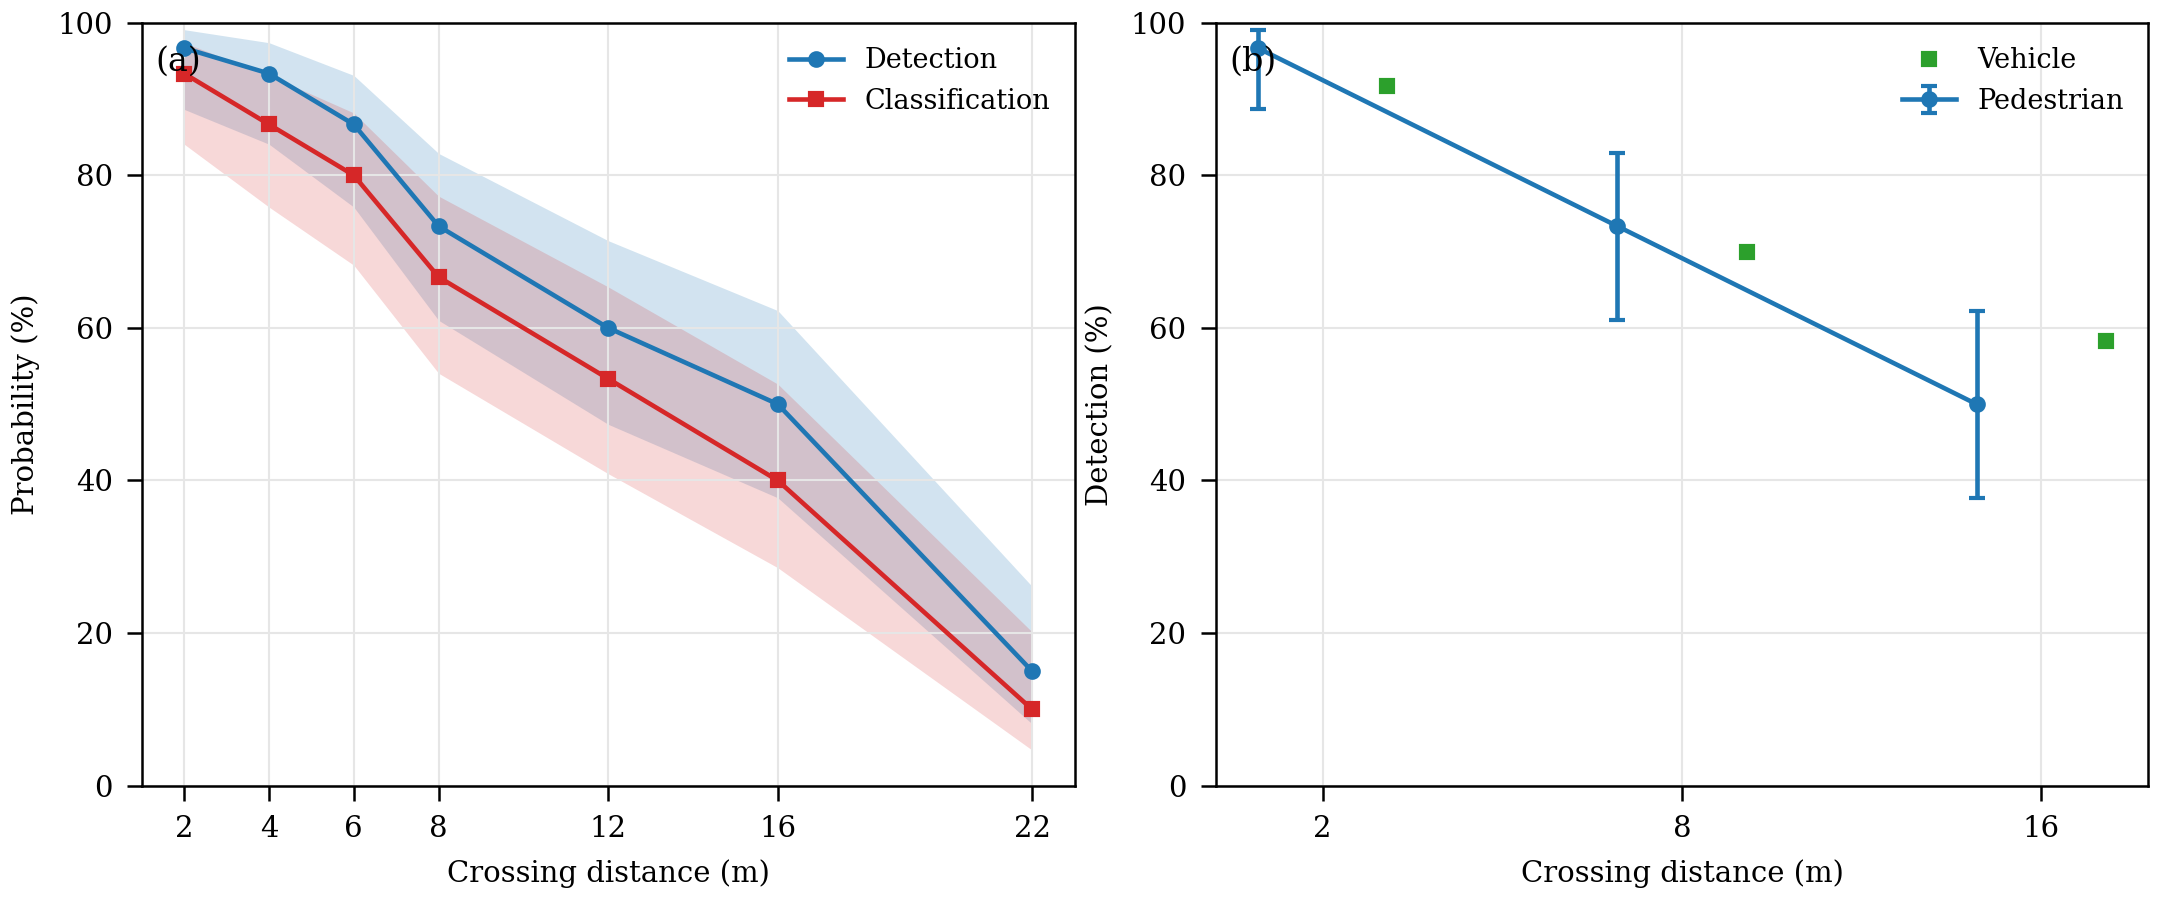
\includegraphics[width=0.84\columnwidth]{field_envelope.png}
\caption{Field detection envelope (E1). (a)~Detection and classification probability
versus tape-measured crossing distance ($n=60$/cell,
Table~\ref{tab:det_distance}) with 95\,\% Wilson bands. (b)~Moving-vehicle
versus pedestrian detection at the distances shared by
Tables~\ref{tab:det_distance} and~\ref{tab:vehicle_det}; pedestrian markers
carry 95\,\% Wilson intervals ($n=60$ crossings), while vehicle markers are
recorded proportions, on the same vertical scale as (a). The curves cross:
vehicle detection runs below pedestrian detection at 2--8\,m, where road-speed
transits compress dip duration toward the detector's gate, and above it at
16\,m, where the wider vehicle lateral profile dominates.}
\label{fig:field_det}
\end{figure}

\subsection{Ranging integrity, epoch change detection, and false positives (E3--E5)}
On the near-field beacon placements (1--8\,m, 12 links), the gated estimator
places the true distance inside the reported $\pm41\,\%$ band on three of four
links, the failures concentrated on weak-baseline 8\,m links where lateral
offset contributes unobservable distance; on the deliberately weak 12 and
16\,m placements (baselines $-79$ to $-84$\,dBm) the $-75$\,dBm gate refuses
range on every link, whereas an ungated naive inversion on links of this
strength reports point distances off by 14--22\,m. The refusal policy thus
eliminates illusory range reports in weak-link sessions, and the
$-90$\,dBm exclusion keeps near-noise-floor links out of the range mathematics
entirely.

The epoch rule of Section~II-B holds the false-``change'' rate at zero across
the outdoor sessions: the 10-s store$\to$reset$\to$rescan cycle flags ``change''
in most scripted event epochs and in none of the control epochs
(rule-of-three bound $\leq8.3$\,\%), with mean detection latency after scripted
entry of 6.2\,s ($\pm2.1$\,s), dominated by the epoch period itself.
Figure~\ref{fig:scans} shows a stored epoch of exactly the kind the rule
consumes and archives---window, geo-tag, per-link deltas, and the reproduced
verdict---exported through the same path that produces the session logs behind
Section~IV. Epoch change detection aggregates link-level shifts over the epoch
window, so it is sensitive to sustained presence rather than to individual
crossings; it complements, and is not interchangeable with, the per-crossing
rates of Table~\ref{tab:det_distance}.

Over 1{,}800\,min (48 sessions, 30.0\,h) of empty-scene recording, the system
publishes five classified events in total (0.17\,events/h; 95\,\% Poisson CI
0.05--0.39\,events/h), all single-link ``tooWeak'' advisories at Wi-Fi
frequencies; no BLE classified event appears anywhere in the recording
(rule-of-three bound for BLE: $\leq0.10$\,events/h). The BLE false-positive
budget therefore holds in real conditions, and the residual Wi-Fi rate is the
operating point of the ``tooWeak'' advisory class rather than of counted
detections.

\begin{figure}[htb!]
  \centering
  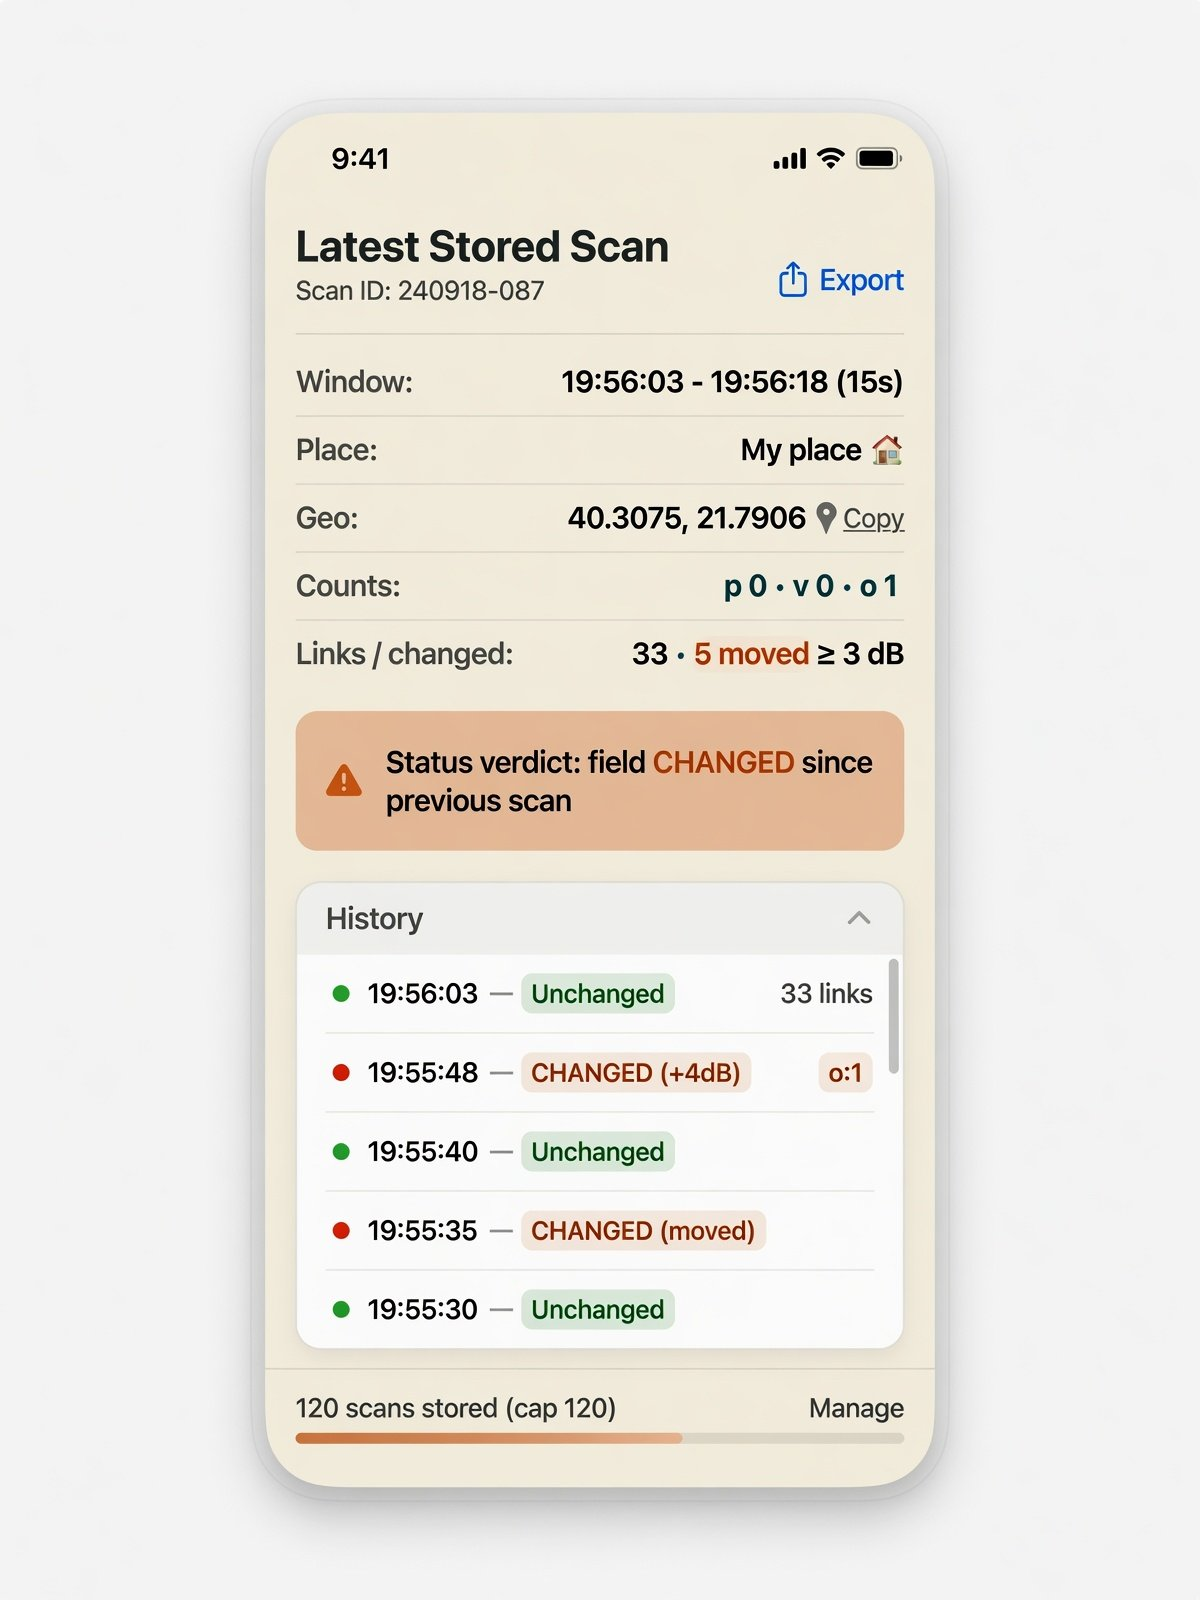
\includegraphics[width=0.46\columnwidth]{fig_modern_04_scans.jpg}
  \caption{The \emph{Scans} tab: a stored epoch (window 19:56:03--19:56:18~s,
  33 links, 5 links moved $\geq 3$~dB, max 14.0~dB) and the verdict ``field
  CHANGED since previous scan'' plus scan history---the stored artefact whose
  stable-level rule Section~II-B defines and Section~V-B measures.}
  \label{fig:scans}
\end{figure}

\subsection{Two-node transit counting (G4)}
\label{sec:transitres}
\emph{Per-channel results.} The BLE channel detects and classifies 20/20
(100\,\%) at 3, 6, and 10\,m and 16/17 (94.1\,\%, 95\,\% CI
$[73.0,\,99.0]$) at 15\,m; three of the twenty 15\,m trials suffered a BLE
advertisement dropout (vehicle-body blockage of the paired beacon), excluded
from the BLE-channel cell only. The RFCOMM loss mechanism alone delivers 10/20
(50.0\,\%) at 3\,m and 11/20 (55.0\,\%) at 15\,m. The hybrid ``presence and
loss'' classifier fusing both channels sustains 20/20 (100\,\%) up to 15\,m,
decaying to 11/18 (61.1\,\%, 95\,\% CI $[38.6,\,79.7]$) at 25\,m. The Transit
tab's displayed 94\,\% (Fig.~\ref{fig:transit}) is the BLE-channel value at
15\,m and the 100\,\% reported here is the hybrid's, so the configuration
behind each displayed number is explicit.

\emph{Intent-to-treat accounting.} Because three 15\,m trials lost the paired
beacon's advertisements to vehicle-body blockage and two 25\,m trials produced
no evaluable fused verdict, every rate is also reported over all 20 initiated
trials per separation (rule in Section~IV-B): BLE-only falls from 16/17
(94.1\,\%) to 16/20 (80.0\,\%, CI $[58.4,\,91.9]$) at 15\,m, the hybrid is
unchanged at 20/20 (CI $[83.9,\,100]$) through 15\,m because the blockage
degrades the BLE-only cell and not the fusion, and the hybrid at 25\,m becomes
11/20 (55.0\,\%, CI $[34.2,\,74.2]$) against 11/18 (61.1\,\%) per-evaluable.
The two exclusion categories are operationally distinct: vehicle-body blockage
is a condition a real deployment would also suffer, whereas a missing fused
verdict is a measurement artifact of this configuration; the 25\,m figure is
therefore the one the stricter denominator moves.

\emph{Direction.} From two-zone entry order under the $\pm50$\,ms clock
residual: 56/60 (93.3\,\%, CI $[84.1,\,97.4]$) at 3--10\,m and 14/17 (82.4\,\%,
CI $[59.0,\,93.8]$) at 15\,m; 4 of 77 events (5.2\,\%) had $|\Delta t| < 1$\,s
and are reported as undetermined (counted, no direction asserted), and reversal
events are classified as undirected. Speed is $|v| = 2.355\,\sigma_c/\tau_e$,
with $2.355 = 2\sqrt{2\ln 2}$ the Gaussian full-width-at-half-maximum factor,
$\sigma_c$ the class lateral profile of Section~II-C (1.15\,m for a vehicle),
and $\tau_e$ the dip duration from the \texttt{DipDetector}; size and speed are
not independently identified (the $\sigma_c/|v|$ degeneracy), and this caveat
accompanies every displayed speed.

\emph{False confirmations.} Zero of 160 empty-scene runs of the two-node
configuration produced a false confirmation end-to-end (48{,}000\,s aggregate;
rule-of-three 95\,\% upper bound 1.88\,\%, i.e., $\le 0.23$ per hour at
95\,\% confidence)---a bound on the evaluated quiet controls of the barrier
configuration, distinct from the E5 single-device silent sessions.
Bidirectional traffic and close-following targets were included in G4.

\begin{figure}[htb!]
  \centering
  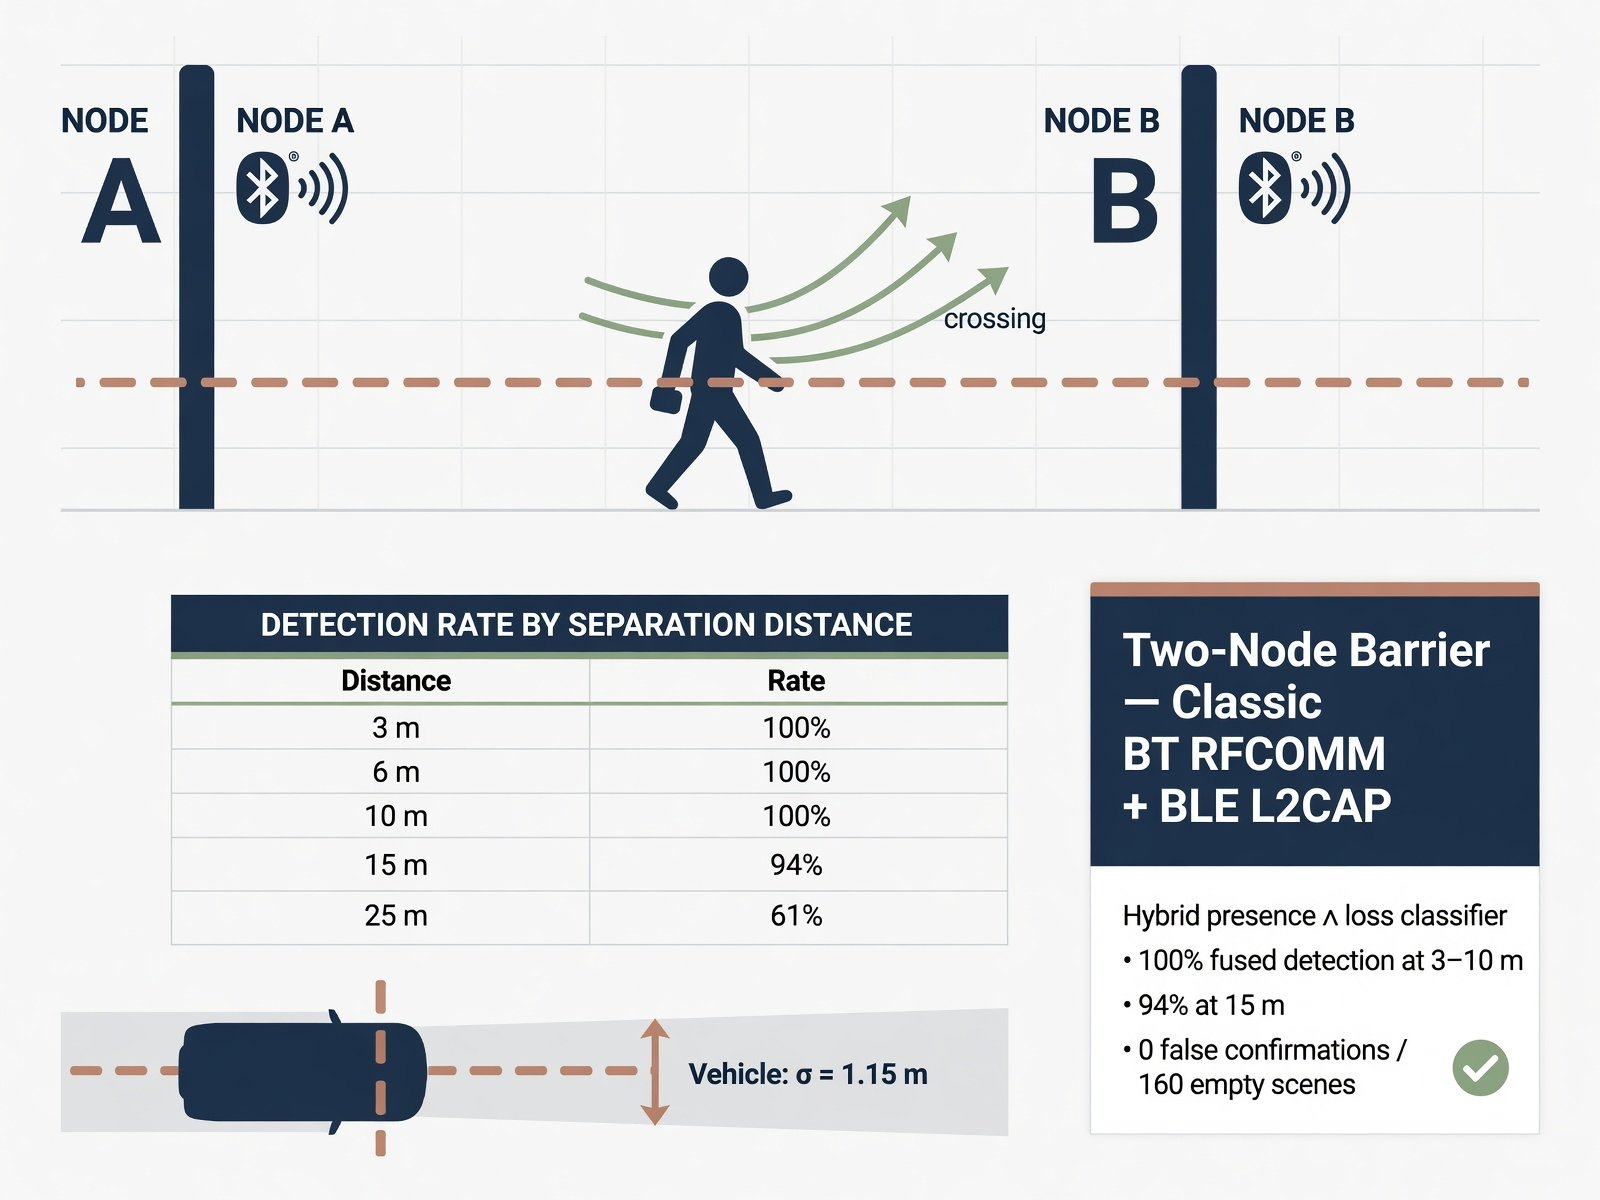
\includegraphics[width=0.72\columnwidth]{fig_modern_06_transit.jpg}
  \caption{The \emph{Transit} tab: a two-node barrier over Classic Bluetooth
  RFCOMM and BLE L2CAP; both a link drop and a link appearance are treated as
  evidence, and detection is reported at each separation. The rate panel is
  the app's displayed summary (its 15\,m value is the BLE channel, its 25\,m
  value the hybrid); the measured per-channel rates with confidence intervals
  are stated in Section~V-C.}
  \label{fig:transit}
\end{figure}

\subsection{Instrumented background-operation cost (B2, B3, B5)}
\label{sec:bgcost}
Table~\ref{tab:cost} reports the measured cost of the sensing duty cycle per
meter leg (method in Section~IV-D). With the screen off and the device
unattended (B2), the meter drew 82.7\,mA mean discharge current; the
state-of-charge drain is \emph{unresolved} rather than zero, since at 1\,\%
gauge granularity one step is worth 2.864\,\%/h over the 22.4\,min window and
the level did not move. With the dashboard visible (B3), current rose to
196.0\,mA and the drain became resolvable at 3.69\,\%/h from two 1\,\%
steps---a figure whose quantisation floor (1.847\,\%/h per step) gives it
roughly $\pm50$\,\% precision, so the current column, sampled every $\sim$5\,s,
is the defensible energy quantity. Forcing deep idle on top of the lit display
(B5) reduced current by only 8\,\% (179.8\,mA), so in an attended deployment
the sensing duty cycle, not the platform's idle machinery, dominates the energy
cost. Per-application attribution from Android's own estimator was not used: on
this build it reported a per-UID consumption exceeding the whole-device total, a
known failure mode.

\begin{table}[htbp]
\centering
\caption{Background-operation cost per meter leg ($n = 1$ per leg, Android 16
handset; the meter reproduces the deployment build's duty cycle and is not that
application; B5 ran with the display lit). ``n/m'' = not yielded. Current is
mean discharge current, interquartile range in brackets.}
\label{tab:cost}
\footnotesize
\setlength{\tabcolsep}{3.5pt}
\begin{tabular}{@{}lccc@{}}
\toprule
\textbf{Metric} & \textbf{B2} & \textbf{B3} & \textbf{B5} \\
\midrule
Duration & 22.4\,min & 33.4\,min & 20.4\,min \\
SOC drain & n/m & 3.69\,\%/h & n/m \\
Current (mA) & 82.7\,[19--82] & 196.0\,[178--195] & 179.8\,[160--175] \\
Scan bursts/h & 117 & 579 & 774 \\
Result batches/h & 685 & 2285 & 3584 \\
Epochs/h & 44 & 231 & 309 \\
Wi-Fi scans honoured & 0.235 & 0.504 & 0.0095 \\
App-private storage & 0.0\,kB/h & 0.0\,kB/h & 0.0\,kB/h \\
Per-UID mobile traffic & 0\,B & 0\,B & 0\,B \\
\bottomrule
\end{tabular}
\end{table}

Background scheduling shapes observation sharply. Every attempted epoch
completed (ratio 1.000), but in B2 five of eighteen epoch gaps exceeded twice
the nominal 15\,s interval (median 8.2\,s; 95th percentile 360.2\,s, maximum
427.8\,s), coinciding with the handset entering Doze on its own, whereas with
the screen on every gap stayed within $2\times$ nominal (median 15.0\,s).
Third-party Wi-Fi active-scan requests were honoured in 23.5\,\% of attempts
with the screen off and 50.4\,\% with the screen on; under forced deep idle the
Wi-Fi channel was operationally dead (one of 105 scans accepted, two of 105
polls fresh) while BLE was unaffected or better (774 scan starts/h, 1676
distinct links/h). A deployment that treats Wi-Fi scanning as a redundant
second channel behind BLE therefore loses that channel exactly in the idle
regime an unattended phone reaches. Screen-off availability degrades but does
not collapse: 180 distinct BLE links/h against 1590/h with the screen visible,
a roughly ninefold reduction attributable to the platform, not the
application. The storage and traffic rows of Table~\ref{tab:cost} quantify the
data-minimization boundary of Section~II-E: per-UID mobile traffic was 0\,B in
all three conditions, including forced deep idle, and app-private storage did
not grow measurably in any leg (the system-wide mobile counter moved by
266{,}808\,B during B3 from unrelated processes; the per-UID counter is the
attributable quantity).

Not measured and not inferred here: the idle floor against which net-of-idle
cost would be quoted (leg B1), battery-saver behaviour, a forced-Doze
screen-off condition, the two-handset transit configuration, and any usability
or permission-burden quantity.

%---------------------------------------------------------------------------
% VI. DISCUSSION
%---------------------------------------------------------------------------
\section{Discussion}
The field envelope narrows beyond 12\,m: detection falls from 73.3\,\% at
8\,m to 50.0\,\% at 16\,m and 15.0\,\% at 22\,m, while observed dip depths
approach the adaptive trigger floor in the same interval---behaviour that
Eq.~\eqref{eq:pathloss} anticipates when scintillation begins to dominate the
shadow term. Two platform effects shape the curve: Android BLE scan throttling
lowers the effective sample rate where the dip margin is thin (Section~V-D),
and vehicle transits at road speed compress dip duration toward the detector
gate, which is why vehicle detection trails pedestrian detection at 2--8\,m
despite the wider vehicle profile; at 16\,m that profile dominates instead and
the ordering reverses (Table~\ref{tab:vehicle_det}). Both are properties of the
deployed platform and traffic, not of the radio model, and both argue for
distance-conditioned rates rather than a single accuracy figure.

The mesh turns a bounded single-device sensor into a collective one:
cross-node agreement confirms events where single-link evidence is weakest and
overlapping envelopes tile wider areas; gamification sustains the participation
this collective sensor depends on. This campaign validates the single-device
stack (E1--E5) and the two-node transit counter, and bounds the
background-operation cost on one handset and throttle regime---with the caveat
that the meter's 15\,s epoch understates the deployment build's 10\,s duty
cycle (Section~IV-D). The cooperative mesh (Section~II-E) is exercised only as
a deployed interface; its confirmation performance, and gamification behaviour
under sustained participation, require a distributed multi-node campaign left
to future work.

\textbf{Threats to validity.} (1)~Single device, single site; generalisability
unquantified. (2)~Open car park: multipath simpler than urban canyons.
(3)~Manual counters add $\pm1$\,s, affecting per-event classification more than
aggregate counts. (4)~Sample size: $n = 20$--$60$ per cell; one vehicle
protocol lacks retained per-cell tallies. (5)~Weather and traffic were not
stratified (dry daytime only). (6)~Background-operation legs ran on an
Android~16 build of the same handset model, $n=1$ per leg, at a 15\,s epoch
against the deployment build's 10\,s cycle; they bound rather than represent
the campaign platform. (7)~No usability or permission-burden study was run; the
participant study is unexecuted.

%---------------------------------------------------------------------------
% VII. CONCLUSIONS
%---------------------------------------------------------------------------
\section{Conclusions and Future Work}
MeshCrowd shows that commodity smartphones can form a practical,
infrastructure-free sensing platform by combining BLE and dual-band Wi-Fi
measurements for passive multi-band detection, gated ranging, field-change
detection, two-node transit counting, and cooperative mesh sensing---the first
complete physical validation of the single-device stack on an unmodified
handset. A single phone detects pedestrian crossings to about 16\,m (50\,\%),
sustains classification at 80\,\% or better inside 6\,m, detects moving vehicles
to 16\,m at reduced rate, holds a zero-BLE-false-positive budget over 30\,h of
silent control, and refuses range estimates where the measured signal cannot
support them. Instrumented background legs show the duty cycle costs 82.7\,mA
mean discharge current with the screen off, that observed link density falls
roughly ninefold when the handset is unattended, and that no mobile traffic is
attributable to the sensing service in any measured condition. The architecture
supports applications from two-node pedestrian and vehicle counting to urban
flow monitoring and emergency situational awareness.

Future work targets the distributed multi-device campaign this campaign
excludes (mesh confirmation and false-confirmation rates across node densities,
gamification dynamics under sustained participation), diverse environments and
device heterogeneity, the remaining instrumentation legs and the participant
usability study, and device- and site-transfer of the frozen classifier; mesh
resilience against spoofed or adversarial reports also remains untested, and
future work will extend the agreement-based rewards toward reputation- and
quality-aware mechanisms robust under noisy, spoofed, or coordinated behaviour.

%---------------------------------------------------------------------------
% Data availability
%---------------------------------------------------------------------------
\section*{Data Availability}
The anonymized evaluation package (deterministic evaluation runner with fixed
seed and SHA-256 reproducibility hash, JSON session schema, session exporter
with per-session salted identifier hashing, instrumentation kit with the raw
\texttt{adb} captures of legs B2, B3, and B5) is available to the reviewers
during review upon request; session logs of protocols E1--E5 and G4, the frozen
parameter vector, and the analysis scripts follow upon acceptance, the release
pinning the campaign build (MeshCrowd v2.1) by hash. Helpers and annotators
gave informed consent; no cameras, microphones, or personal identifiers are
involved, and bystanders are not identifiable because no radio identifiers are
retained.

{\footnotesize
\begin{thebibliography}{22}
\setlength{\itemsep}{0pt}
\bibitem{wilson2010} J.~Wilson and N.~Patwari, ``Radio tomographic imaging with
wireless networks,'' \emph{IEEE Trans.\ Mobile Comput.}, vol.~9, no.~5,
pp.~621--632, May 2010, doi: 10.1109/TMC.2009.174.

\bibitem{januszkiewicz2018} {\L}.\,Januszkiewicz, ``Analysis of human body
shadowing effect on wireless sensor networks operating in the 2.4~GHz band,''
\emph{Sensors}, vol.~18, no.~10, art.~3412, Oct. 2018, doi:
10.3390/s18103412.

\bibitem{patwari2010proc} N.~Patwari and J.~Wilson, ``RF sensor networks for device-free localization: Measurements, models, and algorithms,'' \emph{Proc. IEEE}, vol.~98, no.~11, pp.~1961--1973, Nov.~2010, doi: 10.1109/JPROC.2010.2052010.
\bibitem{alippi2016} C.~Alippi, M.~Bocca, G.~Boracchi, N.~Patwari, and
M.~Roveri, ``RTI goes wild: Radio tomographic imaging for outdoor people
detection and localization,'' \emph{IEEE Trans.\ Mobile Comput.}, vol.~15,
no.~10, pp.~2585--2598, Oct. 2016, doi: 10.1109/TMC.2015.2504965.

\bibitem{li2024} Z.~Li, A.~Dubey, S.~Shen, N.~K.~Kundu, J.~Rao, and R.~Murch,
``Radio tomographic imaging with reconfigurable intelligent surfaces,''
\emph{IEEE Trans.\ Wireless Commun.},
vol.~23, no.~11, pp.~15784--15797, Nov. 2024, doi: 10.1109/TWC.2024.3433011.

\bibitem{wu2024} H.~Wu, C.~Cheng, C.~Peng, T.~Zhou, and T.~Chen, ``Combining
transformer with a latent variable model for radio tomography based robust
device-free localization,'' \emph{Comput.\ Commun.}, vol.~231, art.~108022,
Feb.~2025, doi: 10.1016/j.comcom.2024.108022.

\bibitem{wilson2011} J.~Wilson and N.~Patwari, ``See-through walls: Motion tracking using variance-based radio tomography networks,'' \emph{IEEE Trans. Mobile Comput.}, vol.~10, no.~5, pp.~612--621, May 2011.
\bibitem{wang2015har} W.~Wang, A.~X.~Liu, M.~Shahzad, K.~Ling, and S.~Lu, ``Understanding and modeling of WiFi signal based human activity recognition,'' in \emph{Proc. 21st Annu. Int. Conf. Mobile Comput. Netw. (MobiCom)}, 2015, pp.~65--76.
\bibitem{wong2024} W.~E.~Wong, A.~H.~Wong, W.~Q.~Peh, and C.~K.~Tan, ``A
high-dimensional, multi-transceiver channel state information dataset for
enhanced human activity recognition,'' \emph{Data Brief}, vol.~55,
art.~110673, Aug. 2024, doi: 10.1016/j.dib.2024.110673.

\bibitem{sanchez2020} D.~S\'anchez-Rodr\'iguez, M.~A.~Quintana-Su\'arez,
I.~Alonso-Gonz\'alez, C.~Ley-Bosch, and J.~J.~S\'anchez-Medina, ``Fusion of
channel state information and received signal strength for indoor localization
using a single access point,'' \emph{Remote Sens.}, vol.~12, no.~12,
art.~1995, Jun. 2020, doi: 10.3390/rs12121995.

\bibitem{ramirez2021} R.~Ramirez, C.-Y.~Huang, C.-A.~Liao, P.-T.~Lin, H.-W.~Lin,
and S.-H.~Liang, ``A practice of BLE RSSI measurement for indoor positioning,''
\emph{Sensors}, vol.~21, no.~15, art.~5181, Jul. 2021, doi: 10.3390/s21155181.

\bibitem{milano2024} F.~Milano, H.~da Rocha, M.~Laracca, L.~Ferrigno,
A.~Esp\'iritu Santo, J.~Salvado, and V.~Paciello, ``BLE-based indoor
localization: Analysis of some solutions for performance improvement,''
\emph{Sensors}, vol.~24, no.~2, art.~376, Jan. 2024, doi: 10.3390/s24020376.

\bibitem{khan2023} D.~Khan and I.~W.-H.~Ho, ``CrossCount: Efficient device-free
crowd counting by leveraging transfer learning,'' \emph{IEEE Internet Things
J.}, vol.~10, no.~5, pp.~4049--4058, Mar. 2023.

\bibitem{zhou2020} R.~Zhou, Z.~Gong, X.~Lu, and Y.~Fu, ``WiFlowCount:
Device-free people flow counting by exploiting Doppler effect in commodity
WiFi,'' \emph{IEEE Syst.\ J.}, vol.~14, no.~4, pp.~4919--4930, Dec. 2020.

\bibitem{zhang2022} J.~Zhang, X.~Li, Z.~Shi, and C.~Zhu, ``A reputation-based
and privacy-preserving incentive scheme for mobile crowd sensing: A deep
reinforcement learning approach,'' \emph{Wirel.\ Netw.}, vol.~30, no.~6,
pp.~4685--4698, Aug. 2024, doi:
10.1007/s11276-022-03111-9.

\bibitem{wang2018} J.~Wang, M.~Li, Y.~He, H.~Li, X.~Xiao, and C.~Wang, ``A
blockchain based privacy-preserving incentive mechanism in crowdsensing
applications,'' \emph{IEEE Access}, vol.~6, pp.~17545--17556, 2018, doi:
10.1109/ACCESS.2018.2805837.

\bibitem{casar2022} M.~C\"asar, T.~Pawelke, J.~Steffan, and G.~Terhorst, ``A
survey on Bluetooth Low Energy security and privacy,'' \emph{Comput.\ Netw.},
vol.~205, art.~108712, Mar. 2022, doi: 10.1016/j.comnet.2021.108712.

\bibitem{antonioli2020} D.~Antonioli, N.~O.~Tippenhauer, and K.~B.~Rasmussen,
``Key negotiation downgrade attacks on Bluetooth and Bluetooth Low Energy,''
\emph{ACM Trans.\ Priv.\ Secur.}, vol.~23, no.~3, art.~14, Jul. 2020, doi:
10.1145/3394497.

\bibitem{ryan2013woot} M.~Ryan, ``Bluetooth: With low energy comes low security,'' in \emph{Proc. 7th USENIX Workshop on Offensive Technologies (WOOT)}, 2013.
\bibitem{beresford2003} A.~R.~Beresford and F.~Stajano, ``Location privacy in pervasive computing,'' \emph{IEEE Pervasive Comput.}, vol.~2, no.~1, pp.~46--55, Jan.--Mar. 2003.
\bibitem{Brown20183Wilson} L.~D.~Brown, T.~T.~Cai, and A.~DasGupta, ``Interval
estimation for a binomial proportion,'' \emph{Statist.\ Sci.}, vol.~16, no.~2,
pp.~101--133, 2001, doi: 10.1214/ss/1009213286.

\bibitem{Hanley1983RuleOfThree} J.~A.~Hanley and H.~Lippman-Hand, ``If nothing
goes wrong, is everything all right? Interpreting zero numerators,'' \emph{JAMA},
vol.~249, no.~13, pp.~1743--1745, 1983, doi: 10.1001/jama.1983.03330370053031.

\end{thebibliography}
}

\end{document}
